\subsection{Deep Learning} \label{sec:background-deep-learning}

One of the factors that determines the effectiveness of neural network models is how the features that define the model's inputs and outputs are represented. For example, to construct a model that learns to classify objects in an image, the images would traditionally be pre-processed to extract certain features like edges before being fed into the neural network model. The quality of the feature engineering process significantly affects the outcome of the classification. Certain application domains do not have automated algorithms that can pre-process inputs, in which case feature engineering must be done manually\cite{Goodfellow-et-al-2016}.

To avoid the effort and error introduced by manual feature engineering, machine learning models are adapted to learn feature representations. This usually results in models that perform better than the ones that depended on manually specified features. The ability of these machine learning models to identify the important aspects of the application domain, such as facial recognition, depend on the ability of such models to disentangle the factors of variation that comprise the problem\cite{Bengio:2009:LDA:1658423.1658424}.

This process of separating the important factors from those that are not is considered difficult. In order to capture the complexity of such tasks, we construct representation learning models that are several layers deep. Constructing models in such a layered topology allows the models to represent the application domain in terms of a hierarchy of concepts, with each concept defined through its relation to simpler concepts\cite{Goodfellow-et-al-2016}. Each layer represents the model's understanding of a particular level of abstraction with each level being more abstract than the layer below\cite{Bengio:2009:LDA:1658423.1658424}. This borrows from the fact that our nervous system processes sensory input via a multi-layer hierarchy of neurons\cite{DBLP:journals/corr/abs-1203-2990}. For example, a model that can be used to identify objects in an image can be constructed in several layers. One layer learns to identify edges, the next layer learns to identify simple shapes all the way up to the final layer (output layer) that makes the actual classification.

Figure \ref{fig:feature-representation-learning} shows an example of what the weights of each layer of a deep neural network would learn to represent. Raw pixels are presented as input to the network, the first hidden layer then detects the edges in the image, the second layer detects parts of an object and the final hidden layer detects the object. The model then outputs the classification of what it ``sees" in the input image.

\begin{figure}[t]
	\centering
	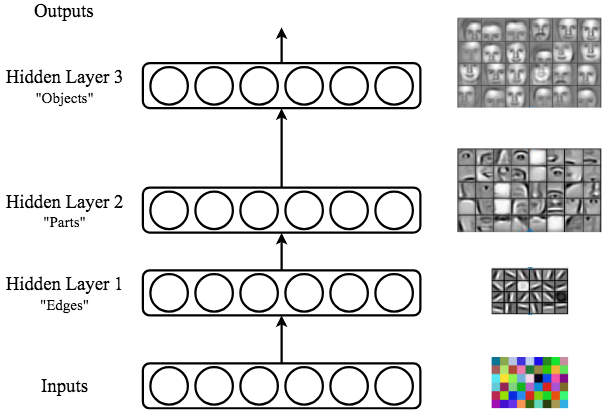
\includegraphics[max width=\textwidth]{feature-representation-learning}
	\caption{Deep feed forward neural network learning to classify objects in an image. Each layer learns to represent a level of abstraction that is more high level than the layer below.}
	\label{fig:feature-representation-learning}
\end{figure}

\subsubsection{The Depth-Breadth Tradeoff}

Besides increasing the representational power of neural network models, empirical evidence also shows that by adding more layers to the neural network architecture the efficiency of the model is also improved. 

The computational complexity of both the feed forward phase and the backpropagation phase of a feed forward neural network is dependent on the number of parameters (weights) that define the model. By having an architecture that is as compact as possible, but at the same time has sufficient complexity to represent the target function, we reduce the required number of weights and therefore have a better performing model.

Bengio 2009 discusses that if a function can be compactly represented by a deep architecture, it might need an exponentially large architecture to be represented by an insufficiently deep one\cite{Bengio:2009:LDA:1658423.1658424}. Therefore, deep architectures help in discovering compact architectures that significantly reduce the computational complexity of the models.

\subsubsection{GPU Training}

The accuracy of trained neural network models depends on the number and variety of the training examples provided. The more factors of variation the problem exhibits the more examples the model will need in order to capture the complexity of the problem. It is therefore important to develop methods to improve the speed of training, especially for difficult problems. One way to accomplish that is by using parallelism. This refers to using more than one processor to train a single model.

There are two forms of parallelizing neural networks. The first is model parallelism, which refers to partitioning the neurons that make up the model onto several processors. Communication is needed so that the outputs of one partition can be fed into another partition. The second type of parallelism is called data parallelism. Each machine holds a copy of the model and the training data is divided among the copies. Each copy is trained independently and then the weight values are integrated after training\cite{Le15atutorial2}.

Many off the shelf computers incorporate Graphics Processing Units (GPUs) that support General Purpose GPU computing (GPGPU). GPUs can have hundreds and sometimes thousands of processing cores collectively allowing for parallel computing. This makes it convenient and affordable to parallelize machine learning. Some machine learning libraries like TensorFlow support running models on GPU powered machines. In this research, we take advantage of GPUs to run our experiments.